%Dokumentenklasse "scrbook" - Erweitert um den Verweis auf die Verzeichnisse und Texteigenschaften
\documentclass[chapterprefix=true, 12pt, a4paper, oneside, parskip=half, listof=totoc, bibliography=totoc, numbers=noendperiod]{scrbook}

% Ränder (Standard bottom ca. 52mm anbzüglich von ca. 4mm für die nach oben rechts gewanderte Seitenzahl)
%Anpassung der Seitenränder
\usepackage[bottom=48mm,left=25mm,right=25mm]{geometry}

% Ränder bei Bedarf zeigen
%\usepackage{showframe}

%Tweaks für scrbook
\usepackage{scrhack}

%Blindtext
\usepackage{blindtext}

%Erlaubt unteranderem Umbrücke captions
\usepackage{caption}

%Stichwortverzeichnis
\usepackage{imakeidx}

%Kompakte Listen
\usepackage{paralist}

%Zitate besser formatieren und darstellen
\usepackage{epigraph}

%Glossar, Stichworverzeichnis
\usepackage[toc, acronym]{glossaries} % Akronyme werden als eigene Liste aufgeführt
\usepackage{acronym}
%Anpassung von Kopf- und Fußzeile
%beinflusst die erste Seite des Kapitels
\usepackage[automark,headsepline]{scrlayer-scrpage}
\automark{chapter}
\ihead{\leftmark}
\chead{}
\ohead{\thepage}
\ifoot*{}
\cfoot[\thepage]{}
\cfoot*{}
\ofoot*{}
\pagestyle{scrheadings}

%Auskommentieren für die Verkleinerung des vertikalen Abstandes eines neuen Kapitels
%\renewcommand*{\chapterheadstartvskip}{\vspace*{.25\baselineskip}}

%Zeilenabstand 1,5
\usepackage[onehalfspacing]{setspace}

%Verbesserte Darstellung der Buchstaben zueinander
\usepackage[stretch=10]{microtype}

%Deutsche Bezeichnungen für angezeigte Namen (z.B. Innhaltsverzeichnis etc.)
\usepackage[ngerman]{babel}

%Unterstützung von Umlauten und anderen Sonderzeichen (UTF-8)
\usepackage{lmodern}
\usepackage[utf8]{luainputenc}
\usepackage[T1]{fontenc}

%Einfachere Zitate
\usepackage{epigraph}

%Verwendung von Akronymen
\usepackage[printonlyused]{acronym}

%Unterstützung der H positionierung (keine automatische Verschiebung eingefügter Elemente)
\usepackage{float} 

%Erlaubt Umbrüche innerhalb von Tabellen
\usepackage{tabularx}

%Erlaubt Seitenumbrüche mit Tabellen
\usepackage{longtable}

%Erlaubt die Darstellung von Sourcecode mit Highlighting
\usepackage{listings}

%Definierung eigener Farben bei nutzung eines selbst vergebene Namens
\usepackage[table,xcdraw]{xcolor}

%Vektorgrafiken
\usepackage{tikz}

%Grafiken (wie jpg, png, etc.)
\usepackage{graphicx}

%Grafiken von Text umlaufen lassen
\usepackage{wrapfig}

%Ermöglicht Verknüpfungen innerhalb des Dokumentes (e.g. for PDF), Links werden durch "hidelink" nicht explizit hervorgehoben
\usepackage[hidelinks,german]{hyperref}

%Einbindung und Verwaltung von Literaturverzeichnissen
\usepackage{csquotes} %wird von biber benötigt
\usepackage[style=alphabetic, backend=biber, bibencoding=ascii]{biblatex}
\addbibresource{references/references.bib}

%-------------------------------Zusätzliche Anpassungen und Modifikationen--------------------------------------------%

%Anpassung der Überschriften
\addtokomafont{disposition}{\rmfamily}

%Zusätzliche Farben
\definecolor{darkgreen}{RGB}{0,100,0}

%Umbenennungen
\renewcommand{\lstlistlistingname}{Quelltextverzeichnis}

%Pluszeichen in der Referenc beim zitieren ausblenden
\renewcommand*{\labelalphaothers}{}

%Anpassugen zur Quelltextdarstellung, kann bei Bedarf überschrieben werden (z.B. wenn unterschiedliche Sprachen zum Einsatz kommen)
\renewcommand{\lstlistingname}{Codeauszug}
\lstset{
	language=Java,
	numbers=left,
	columns=fullflexible,
	aboveskip=5pt,
	belowskip=10pt,
	basicstyle=\small\ttfamily,
	backgroundcolor=\color{black!5},
	commentstyle=\color{darkgreen},
	keywordstyle=\color{blue},
	stringstyle=\color{gray},
	showspaces=false,
	showstringspaces=false,
	showtabs=false,
	xleftmargin=16pt,
	xrightmargin=0pt,
	framesep=5pt,
	framerule=3pt,
	frame=leftline,
	rulecolor=\color{green},
	tabsize=2,
	breaklines=true,
	breakatwhitespace=true,
	prebreak={\mbox{$\hookleftarrow$}}
}

%Anpassungen für das Abkürzungsverzeichnis
\newglossarystyle{dottedlocations}{%
	\glossarystyle{list}%
	\renewcommand*{\glossaryentryfield}[5]{%
		\item[\glsentryitem{##1}\glstarget{##1}{##2}] \emph{##3}%
		\unskip\leaders\hbox to 2.9mm{\hss.}\hfill##5}%
	\renewcommand*{\glsgroupskip}{}%
}

\newcommand{\sieheKapitel}[1]{\glqq {#1}\grqq}
\newcommand{\sieheAbbVerweis}[2]{(siehe Abb. {#1} -- {#2})}
\newcommand{\sieheAbb}[1]{(siehe Abb. {#1})}
\usepackage{chngcntr}
\counterwithout{footnote}{chapter}
%%Titles - Uncomment one section of titles
\usepackage[format=plain, justification=RaggedRight, singlelinecheck=false]{caption}
%%Used for titleGraduation
\makeatletter

\newcommand*{\logoPathL}[1]{\gdef\@logoPathL{#1}}
\newcommand*{\logoWidthL}[1]{\gdef\@logoWidthL{#1}}
\newcommand*{\logoPathR}[1]{\gdef\@logoPathR{#1}}
\newcommand*{\logoWidthR}[1]{\gdef\@logoWidthR{#1}}
\newcommand*{\gradeType}[1]{\gdef\@gradeType{#1}}
\newcommand*{\firstExaminer}[1]{\gdef\@firstExaminer{#1}}
\newcommand*{\secondExaminer}[1]{\gdef\@secondExaminer{#1}}
\newcommand*{\matrikelnr}[1]{\gdef\@matrikelnr{#1}}
\newcommand*{\submitDate}[1]{\gdef\@submitDate{#1}}

\renewcommand*{\maketitle}{
	\begin{titlepage}
		\newgeometry{left=2.5cm,right=2.5cm,top=3.0cm,bottom=2.5cm}
		\begin{center}
			\begin{figure}[h]
				\begin{minipage}[hbt]{6cm}
					\flushleft
					\ifx\@logoPathL\empty
					\else
					\includegraphics[width=\@logoWidthL\textwidth]{\@logoPathL}
					\fi
				\end{minipage}
				\hfill
				\begin{minipage}[hbt]{6cm}
					\flushright
					\ifx\@logoPathR\empty
					\else
					\includegraphics[width=\@logoWidthR\textwidth]{\@logoPathR}
					\fi
				\end{minipage}
			\end{figure}
			\vfill
			{\Large \@title\par}
			\vskip 0.5cm
			{\large \bfseries Projektbericht\par}
			\vskip 0.5cm
			{\large \textbf{Studiengang:}\\ 
			Internationale Medieninformatik}
			\vskip 0.5cm
			{\large \textbf{Betreuer:}\\ 
			Prof. Dr.-Ing. Carsten Busch / Alexander Kramer}
			\vskip 0.5cm
			{\large \textbf{Autor:}\\
			Chris Wodäge\\Matrikelnummer: 560597}
			\vskip 2cm
			{Independent coursework \\ Sommersemester 2018}
			\vfill
			\begin{flushleft}
				\begin{tabular}[t]{rl}
					
				\end{tabular}
			\end{flushleft}
		\end{center}
		\restoregeometry
	\end{titlepage}
}
\makeatother
\logoPathL{} %just leave empty to hide logo
\logoWidthL{0.5}
\logoPathR{resources/1000px-Logo_HTW_Berlin.png} %just leave empty to hide logo
\logoWidthR{1}
\gradeType{}
\secondExaminer{}

%%Used for titleResearchPaper
%\makeatletter

\newcommand*{\firstExaminer}[1]{\gdef\@firstExaminer{#1}}
\newcommand*{\subTitle}[1]{\gdef\@subTitle{#1}}
\newcommand*{\researchPart}[1]{\gdef\@researchPart{#1}}
\newcommand*{\matrikelnr}[1]{\gdef\@matrikelnr{#1}}
\newcommand*{\submitDate}[1]{\gdef\@submitDate{#1}}


\renewcommand*{\maketitle}{
	\begin{titlepage}
		\newgeometry{left=2.5cm,right=2.5cm,top=9.0cm,bottom=2.5cm}
		\begin{center}
			\vfill
			{\Large \@title\par}
			{\normalsize \@subTitle\par}
			\vskip 0.5cm
			{\large \bfseries Forschungsprojekt Teil \@researchPart\par}
			\vskip 0.5cm
			{\large an der}
			\vskip 0.5cm
			{\large Hochschule für Technik und Wirtschaft Berlin\\ Fachbereich 4 - Informatik, Kommunikation und Wirtschaft\\ Studiengang Angewandte Informatik}
			\vfill
			\begin{flushleft}
				\begin{tabular}[t]{rl}
					Betreuer: &\@firstExaminer\\
					\\
					Eingereicht von: &\@author\\
					\ifx\@matrikelnr\empty
					\else
					Matrikelnummer: & \@matrikelnr\\
					\fi
					Datum der Abgabe: & \@submitDate
				\end{tabular}
			\end{flushleft}
		\end{center}
		\restoregeometry
	\end{titlepage}
}
\makeatother
%\subTitle{Ein optionaler Untertitel der Arbeit}
%\researchPart{A}

%%Used by all titles
\title{IndustrialVR -- Erstellung einer Virtual Reality Anwendung mit Unity auf Basis von 3D-CAD Daten.}
\author{Chris Wodäge}
\matrikelnr{s0560597} % just leave empty to hide number
\submitDate{05.10.2015}
\firstExaminer{Max Mustermann}
%%End Titles

\makeindex[title=Stichwortverzeichnis, options=-s indexstyle.ist, intoc]
\indexsetup{level=\chapter*,toclevel=chapter}

\makeglossaries
\loadglsentries{glossary_and_acronyms.tex}
\setacronymstyle{long-short}

\begin{document}

\pagenumbering{alph} %fix for same identifier warning, character is not show in title
\maketitle



% Eigenständigkeitserklärung / Abkürzvz
\null\thispagestyle{empty}
\pagenumbering{Roman}
\addchap{Eigenständigkeitserklärung}

Hiermit versichere ich, dass ich die vorliegende Arbeit selbstständig und nur unter
Verwendung der angegebenen Quellen und Hilfsmittel verfasst habe. Die Arbeit wurde bisher
in gleicher oder ähnlicher Form keiner anderen Prüfungsbehörde vorgelegt.

\vskip 1cm

Berlin, den 28.09.2018

\vskip 1.5cm

Chris Wodäge
\input{chapter/Abkürzungsverzeichnis} 

%Abbildungen
\listoffigures \clearpage

\tableofcontents \newpage
\pagenumbering{arabic}


%%============== Neue Seiten ============== %%
\input{chapter/Einführung} \clearpage
\chapter{Umsetzung}
\section{Datenverarbeitung in CAD}
\label{sec:DatenverarbeitungInCAD}
\subsection{Anwendungsbereiche von CAD}
\label{subsec:AnwendungsbereicheVonCAD}
Die Grundlage dieser Arbeit sowie des Prototypen bilden Daten, welche in 3D-CAD-Programmen erstellt wurden. Daher wird im Rahmen dieser Arbeit CAD als Synonym für 3D-CAD verwendet. Im Gegensatz zu 2D-CAD Systemen können in 3D-CAD Systemen Produkte realer konstruiert werden. Das kann sich positiv auf die Entwicklungszeit auswirken. Kollisionsbetrachtungen ermöglichen eine Fehlererkennung, bevor das erste Teil gefertigt wird.\footnote{Vgl. Dipl. Ing. (FH) Bettina Clauß, Helmut Prof. Dr.-Ing. von Eiff (2013): \textit{CAD Grundkurs}. Hochschule Esslingen, S. 2.} Es ist möglich in CAD anhand von Materialeigenschaften physikalische Eigenschaften wie z.B. Festigkeit, Elastizität etc. zu simulieren. Aufgrund dieser Flexibilität sind CAD-Programme heute in fast allen technischen Zweigen vertreten, darunter Architektur, Bauingenieurwesen, Maschinenbau, Elektrotechnik bis hin zur Zahntechnik.\footnote{Vgl. Wikipedia  (2018): \textit{CAD}.\newline
\url{https://de.wikipedia.org/w/index.php?title=CAD&oldid=178934444},\newline 
abgerufen am 23.08.2018.}


\subsection{3D-Modellierung in CAD}
\label{subsec:3D-ModellierungInCAD}
In einer 3D-Umgebung werden Modelle in dreidimensionaler Form modelliert und persistiert. Ein dreidimensionaler Aufbau ermöglicht das Nachbilden einer realitätsnahen Darstellung, das Rendern aus allen Blickwinkeln und Perspektiven sowie eine bessere räumliche Betrachtung. Das Hauptaugenmerk des Ingenieurs liegt dabei vor allem auf Funktionalitäten wie dem technischen Zeichnen, die Erstellung von Arbeitspläne, Montage- und Bedienungsanleitungen oder der technisch visuellen Darstellung, wie der Kollisionsbetrachtung oder der
Zusammenbau-, Einbau- und Montageuntersuchungen. 
Die in dieser Arbeit thematisierte Betrachtung bezieht sich vor allem auf die Nutzung außerhalb der CAD-Umgebung.  Der Vollständigkeit werden nachfolgend alle rechnerinternen Repräsentationen die in CAD vorliegen betrachtet.

\begin{itemize}
\item \textbf{Kantenmodelle:} Kantenmodelle (auch Drahtgitter oder Wireframe) repräsentieren ein Objekt anhand von Kanten. Diese Darstellung enthält keinerlei Informationen über die Flächen oder das Volumen eines Körpers. Kantenmodelle dienen häufig als Hilfsgeometrie, zu Erzeugung von Flächen oder als Darstellungsart von Volumen- oder Flächenmodellen.

\item \textbf{Flächenmodelle:} Als Flächenmodelle werden \glqq hohle\grqq\ Objekte bezeichnet, deren äußere Form durch Flächen beschrieben wird. Eine intuitive Anpassung der Objekthülle ist mit Hilfe von Kontrollpunkten oder Kontrollnetzen ohne Einschränkung möglich. Unter Zuhilfenahme von analytisch beschreibbarer (Translationsflächen, Regelflächen) sowie analytisch nicht beschreibbarer Flächen (B-spline-, NURBS-Flächen) lassen sich jegliche Formen modellieren.

\item \textbf{Volumenmodelle:} Unter Volumenmodelle versteht man Körper, die neben einer Hülle auch eine Materialdichte besitzen, woraus das System automatisch eine Masse interpretiert. Auf diese Weise bleibt die geometrische Konsistenz bei Manipulation des Objektes erhalten. Aufgrund dieses zusätzlichen Parameters kann ein hoher Grad an Automatisierung sichergestellt werden. Es können Eigenschaften wie Trägheit, Schwerpunkt, Gewicht etc. durch das CAD-System automatisch abgeleitet und als Parameter für Simulationen übergeben werden.  
\end{itemize}

Auf alle beschriebenen Modelle lassen sich räumliche Operationen wie Translation, Rotation und Skallierung anwenden. Zusätzlich existieren für jedes Modell spezielle Werkzeuge um diese zu verformen, zu zerschneiden, zu verdrehen oder anderweitig zu manipulieren.\footnote{Vgl. Wikipedia  (2018): \textit{CAD}.\newline
\url{https://de.wikipedia.org/w/index.php?title=CAD&oldid=178934444},\newline 
abgerufen am 23.08.2018.} 

\subsection{Datei- und Exportformate in CAD}
\label{subsec:Datei-undExportformateInCAD}



\clearpage

\section{Aufbereitung der 3D-CAD Daten}
\label{sec:AufbereitungDer3D-CADDaten}



\subsection{Analyse des CAD-Exports}
\label{subsec:AnalyseDesCAD-Exports}
Bevor das aus CAD exportierte Modell in Unity importiert wird sollte selbiges vorher in einem geeigneten 3D-Programm überprüft werden. Für diesen Zweck habe ich auf Autodesk Maya zurückgegriffen. Maya ist eine professionelle Software für Modellierung, Animation und Rendering von 3D Objekten und Szenen.\footnote{Vgl. Autodesk  (2018): \textit{MAYA}.\newline
\url{https://www.autodesk.de/products/maya/overview},\newline 
abgerufen am 30.08.2018.}
\begin{figure}[H]
	\centering
	\captionsetup{width=1\textwidth}
	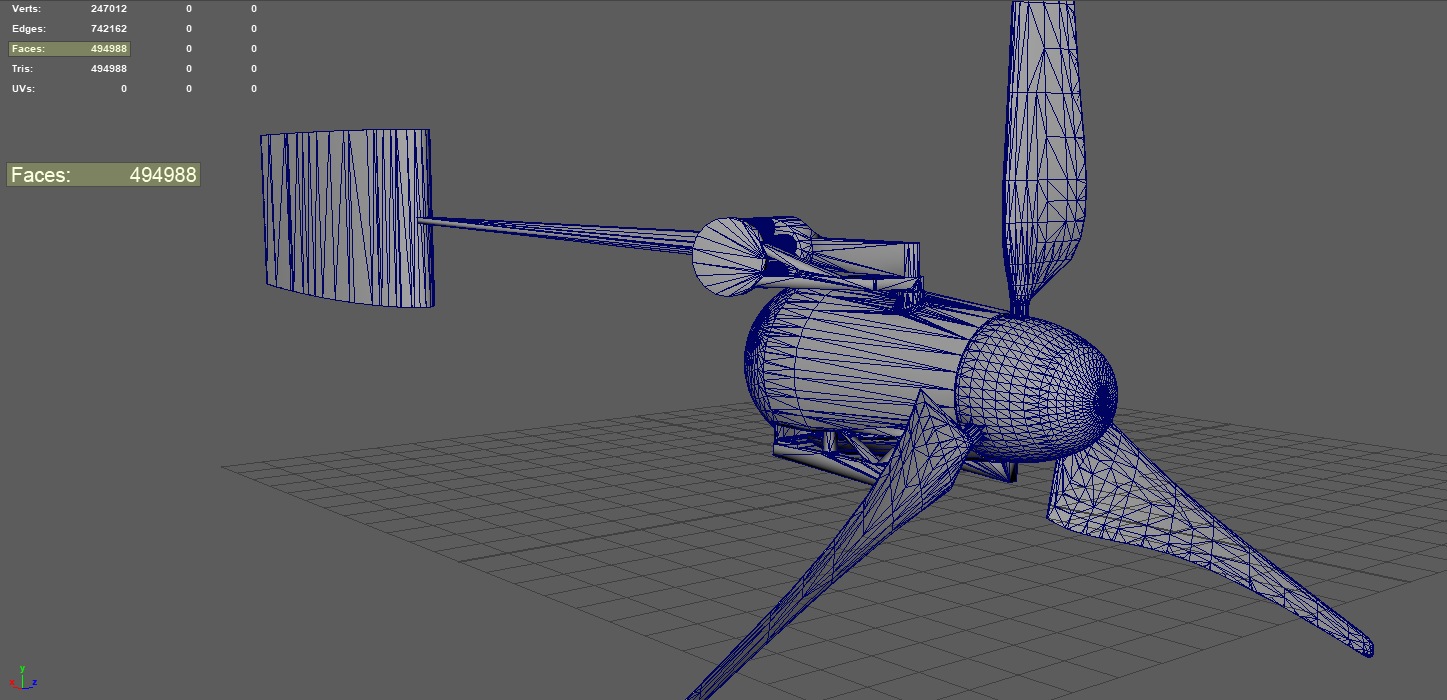
\includegraphics[keepaspectratio, width=1\textwidth]{bildquellen/WEA-Vergleich1}
	\caption{Ergebnis des Exportes der WEA aus der CAD-Anwendung bestehnd aus 494.988 Polygonen.}
	\label{fig:2.1}
\end{figure}
Das importierte Modell \sieheAbb{2.1} weist mehrere Eigenschaften auf, welche es für einen Import sowie eine Weiterverarbeitung in Unity ungeeignet machen. Einerseits besteht das Modell aus nicht ganz 500.000 Polygonen, was für eine Echtzeitanwendung sehr viel ist. 
Andererseits besteht das Modell aus vielen Einzelobjekten, welche zu einem einzigen zusammengefasst sind. Es ist also nicht möglich einzelne Teilobjekte separat mit Materialien auszustatten oder zu Animieren.  
Ferner führt die ungleichmäßige Flächenverteilung zu Darstellungsfehlern beim Shading.



\begin{figure}[H]
	\centering
	\captionsetup{width=1\textwidth}
	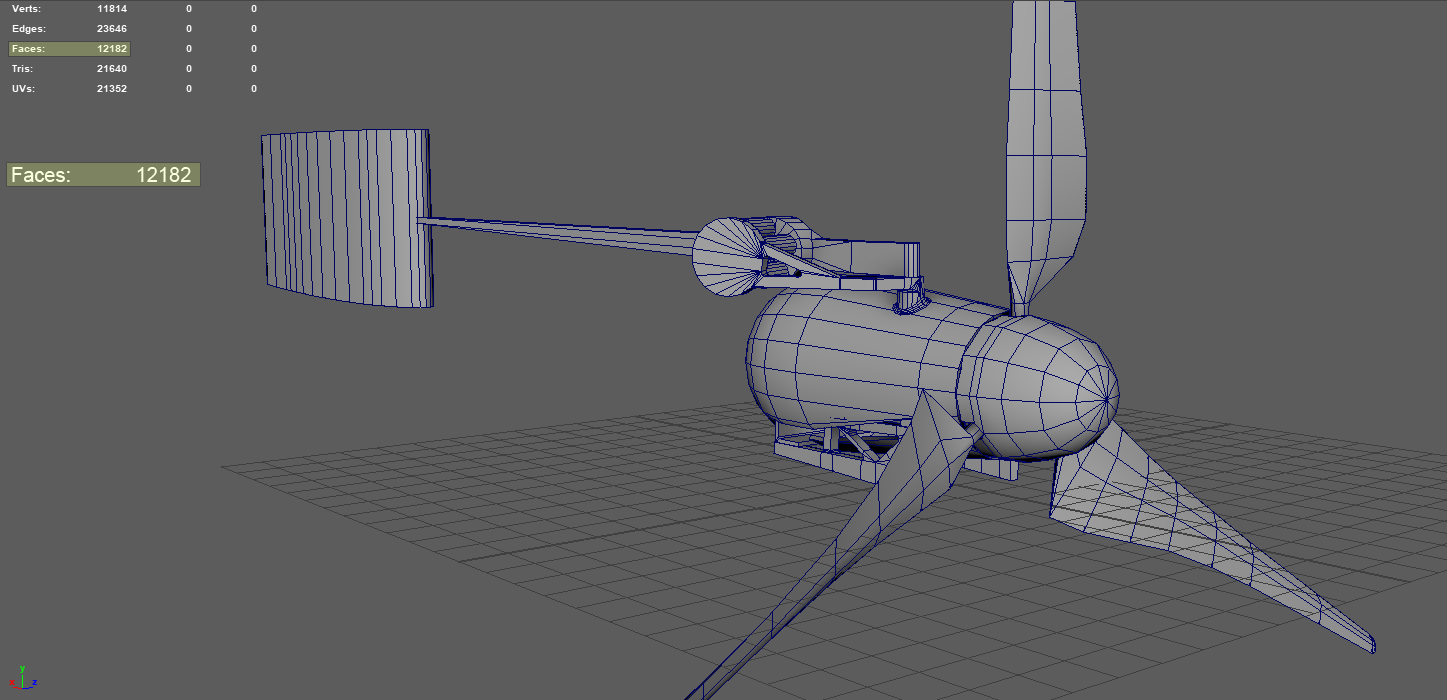
\includegraphics[keepaspectratio, width=1\textwidth]{bildquellen/WEA-Vergleich2}
	\caption{Ergebnis der Retopologisierung bestehend aus 12.182 Polygonen.}
	\label{fig:2.2}
\end{figure} \clearpage


%%\chapter{Beispiele} \label{c:beispiele}

Im Kapitel Beispiele (siehe \autoref{c:beispiele}) werden die möglichen Funktionen und\index{und} Möglichkeiten dies LaTeX-Dokuments demonstriert.

\section{Quelltext}

Nachfolgend der \autoref{lst:helloworld}.

\begin{lstlisting}[caption={Hello World}, captionpos=b, label={lst:helloworld}]
/**
* The HelloWorldApp class implements an application that
* simply prints "Hello World!" to standard output.
*/
class HelloWorldApp {
	public static void main(String[] args) {
		System.out.println("Hello World!"); // Display the string.
	}
}
\end{lstlisting}

\section{Bild}

\begin{wrapfigure}{R}{0.5\textwidth}
	\centering
	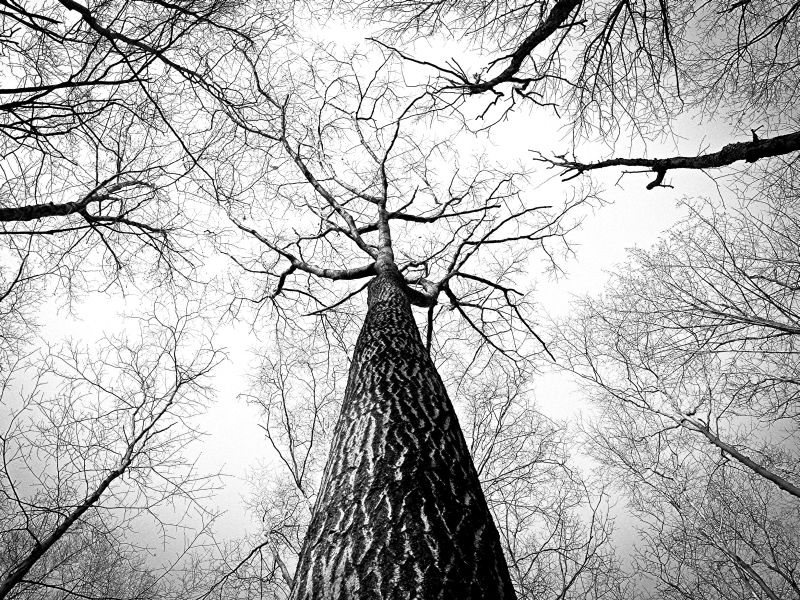
\includegraphics[width=0.5\textwidth]{resources/example}
	\caption{Beispielbild {\cite{PEXELS2015}}}
\end{wrapfigure}

Die rechts zu sehende Grafik demonstriert die Möglichkeiten des Paketes \glqq wrapfig\grqq . Grafiken innerhalb einer \glqq wrapfigure\grqq{} können entweder links oder rechts von Text umlaufen werden.

Die nachfolgende \autoref{img:beispielbild} demonstriert die Darstellung\index{Darstellung} eines \glqq *.jpg\grqq{} Bildes innerhalb des Textes (beim Einfügen kann auf die Endung verzichtet werden, solange der Name einzigartig ist). Zusätzlich enthält dieses einen Untertitel der über das bereits verwendete Label verlinkt werden kann. Der Untertitel\index{Untertitel} erscheint im \gls{abbvz}.

\section{Text Formatierungen und sonstiges}
Dieser Text enthält eine Fußnote\footnote{Fußnoten sind Anmerkungen, die im Druck-Layout aus dem Fließtext ausgelagert werden, um den Text flüssig lesbar zu gestalten.}.

\subsection{Listen}
Listen könne sowohl mit Bullet points als auch mit Zahlen erstellt werden
\begin{itemize}
	\item Eine Liste mit Bullet points
	\item Ein weiteres Element
\end{itemize}

\begin{enumerate}
	\item Eine Liste mit Zahlen
	\item Ein weiteres Element
\end{enumerate}

\subsection{Text Hervorhebungen}
\begin{quote}
	The problem with internet quotes is that you can't always depend on their accuracy \par\raggedleft--- \textup{Abraham Lincoln, 1864}
\end{quote}

"Inspirierende Zitate können mit epigraph eingefügt werden
\epigraph{The problem with internet quotes is that you can't always depend on their accuracy}{Abraham Lincoln, 1864}

Seitenumbrüche können nur direkt nach Text geschrieben werden, sonst lässt sich das Latex nicht mehr compilieren.
\\

\begin{figure}[H]
	\centering
	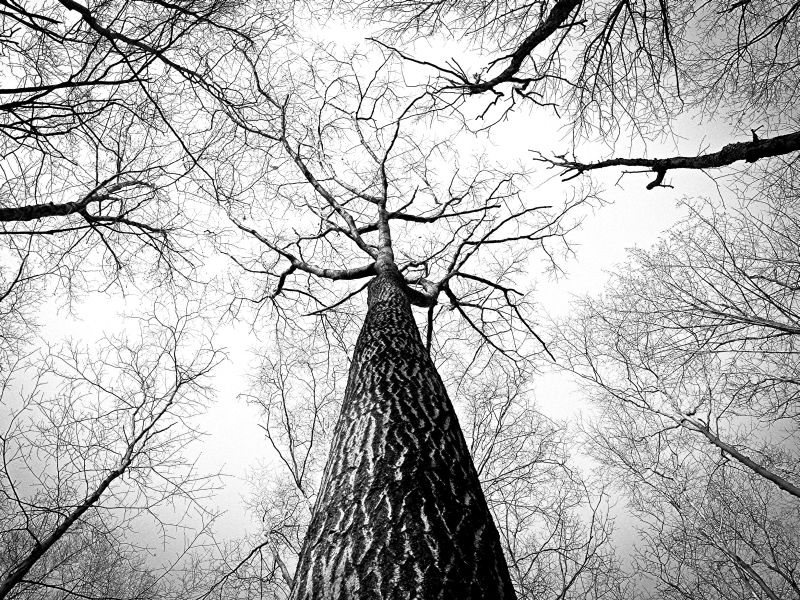
\includegraphics[width=0.7\textwidth]{resources/example}
	\caption{Beispielbild {\cite{PEXELS2015}}}
	\label{img:beispielbild}
\end{figure}

\section{Tabelle}

Nachfolgend \autoref{tbl:DigitalesZertifikat}.

\begin{table}[H]
	\begin{center}
		\renewcommand{\arraystretch}{1.3}
		\begin{tabular}{|l|}
			\hline
			\textbf{Inhaber:}\\
			Alice \\ \hline
			\textbf{Peer (Ersteller):}\\
			Bob \\ \hline
			\textbf{Öffentlicher Schlüssel des Inhabers:}\\
			F2 D2 0E ED FA 4E 9E 0A F2 DD 23 8A 32 44 F3 E9 \\ \hline
			\textbf{Gültigkeit:}\\
			2015-07-01 – 2016-06-30 \\ \hline
		\end{tabular}
	\end{center}
	\caption{Digitales Zertifikat}
	\label{tbl:DigitalesZertifikat}
\end{table}

\section{Long-Table}

Die \glqq Long-Table\grqq kann über definierte Header und Footer über Seitenumbrüche hinweg angezeigt werden.

\begin{longtable}{|l|l|l|l|}
	\hline
	\multicolumn{1}{|c}{\textbf{Version}} & \multicolumn{1}{|c}{\textbf{Codename}} &
	\multicolumn{1}{|c}{\textbf{API}} &
	\multicolumn{1}{|c|}{\textbf{Verteilung}} \\ \hline
	\endfirsthead
	
	\multicolumn{4}{c}{Fortsetzung - Verteilung der Androidversionen (Stand 01.02.2016)}\\ \hline
	\multicolumn{1}{|c}{\textbf{Version}} & \multicolumn{1}{|c}{\textbf{Codename}} &
	\multicolumn{1}{|c}{\textbf{API}} &
	\multicolumn{1}{|c|}{\textbf{Verteilung}} \\ \hline 
	\endhead
	
	\multicolumn{4}{c}{Fortsetzung auf nachfolgender Seite}
	\endfoot
	
	\caption{Verteilung der Androidversionen (Stand: 01.02.2016)}
	\label{tab:androidverteilung}
	\endlastfoot
	
	2.2 & Froyo & 8 & 0.1\%\\ \hline
	2.3.3 - 2.3.7 & Gingerbread & 10 & 2.7\%\\ \hline
	4.0.3 - 4.0.4 & Ice Cream Sandwich & 15 & 2.5\%\\ \hline
	4.1.x & Jelly Bean & 16 & 8.8\%\\ \cline{1-1} \cline{3-4}
	4.2.x &  & 17 & 11.7\%\\ \cline{1-1} \cline{3-4}
	4.3 &  & 18 & 3.4\%\\ \hline
	4.4 & KitKat & 19 & 35.5\%\\ \hline
	5.0 & Lollipop & 21 & 17.0\%\\ \cline{1-1} \cline{3-4}
	5.1 &  & 22 & 17.1\%\\ \hline
	6.0 & Marshmallow & 23 & 1.2\%\\ \hline
\end{longtable}

\section{Literaturverweis}

Weil für die alte\index{alte} und die neue Rechtschreibung verschiedene Trennregeln\index{Trennregeln} gelten, sind Deutsch mit alter Rechtschreibung und Deutsch mit neuer Rechtschreibung zwei verschiedene Sprachen (\cite{Knappen2009}, S. 192).

\section{Onlineverweise}

Siehe Google.de \cite{Google2015}.

\section{Glossar}
Der Glossar enthält die Beschreibung verwendeter Begriffe für das bessere Verständnis gegenüber dem Leser. Beispiele sind: \gls{berlin}, \gls{outsourcing}, \gls{asp}, \gls{policy} und \gls{pcie}.

\section{Abkürzungsverzeichnis}
Das Abkürzungsverzeichnis listet alle verwendeten Abkürzungen auf. Einige Beispiele sind \gls{sas}, \gls{cd}, \gls{lan} und \gls{iso}. Die erneute Verwendung zeigt nur noch die Abkürzung: \gls{sas}, \gls{cd}, \gls{lan} und\index{und} \gls{iso}. \clearpage

%%Verzeichnisse
\pagenumbering{Alph}

%Literatur

\begin{thebibliography}{999}
\label{WindEnergie}
\bibitem{WindEnergie} 
Bundesverband WindEnergie e. V.  (2018): \textit{Funktionsweise von Windenergieanlagen}.\newline
\url{https://www.wind-energie.de/themen/anlagentechnik/funktionsweise/},\newline 
abgerufen am 20.08.2018.

\label{Windpumpsysteme}
\bibitem{Windpumpsysteme} 
Silvio Chemnitz, Sylvio Donner, Florian Hinze, Mats Mojem, Patrick Quandt, Oliver Seidler, Moritz Will, Jens Wuthe (2013): \textit{Windpumpsysteme zur dezentralen Energieversorgung von Abwassersystemen}. TU Berlin.

\label{Bordnetze}
\bibitem{Bordnetze}
Prof. Dr. G. Buch, Prof. Dr. M. Krug (2012): \textit{Kurzskriptum zur Lehrveranstaltung „Elektrische Bordnetze“ im Studiengang Fahrzeugtechnik}. Hochschule München.

\label{CAD}
\bibitem{CAD}
Dipl. Ing. (FH) Bettina Clauß, Helmut Prof. Dr.-Ing. von Eiff (2013):\textit{CAD Grundkurs}. Hochschule Esslingen.

\bibitem{WikiCAD}
Wikipedia  (2018): \textit{CAD}.\newline
\url{https://de.wikipedia.org/w/index.php?title=CAD&oldid=178934444},\newline 
abgerufen am 23.08.2018.


\end{thebibliography}
 \clearpage


% Anhang


\appendix
\renewcommand\thesection{\Alph{section}}
\addchap{Anhang}

\section{Quellen}

\begin{enumerate}[label=A\arabic*]

\item \textit{Windpumpsysteme zur dezentralen Energieversorgung von Abwassersystemen} [PDF]
\item \textit{Kurzskriptum zur Lehrveranstaltung„Elektrische Bordnetze“im Studiengang Fahrzeugtechnik} [PDF]
\item \textit{CAD-Grundkurs} [PDF]
\item \textit{Vergleich von Dateiformatenfür 3D-Modelle} [PDF] 
\item \textit{STL Files and Slicing Software} [PDF] 
\end{enumerate}

\section{Software}

\begin{enumerate}[label=B\arabic*]

\item \textit{IndustrialVR Prototyp} [Unity-Anwendung]
\item \textit{IndustrialVR Projekt} [\url{https://github.com/ChrisWodaege/IndustrialVR.git}]

\end{enumerate} \clearpage

%\listoftables \clearpage
%\lstlistoflistings \clearpage
%\printindex \clearpage
%\printglossary[title={Glossar}] \clearpage
%\printglossary[style=dottedlocations,type=\acronymtype,title={Abkürzungsverzeichnis}] \clearpage
%\printbibliography[heading=bibintoc, keyword={book}, title={Literaturverzeichnis}]\clearpage
%\printbibliography[heading=bibintoc, keyword={online}, title={Onlinequellen}]\clearpage
%\printbibliography[heading=bibintoc, keyword={image}, title={Bildquellen}]\clearpage


\end{document}